\documentclass[14pt]{matmex-diploma}

\usepackage[section]{placeins}

\begin{document}

\filltitle{ru}{
    chair              = {Математическое обеспечение и администрирование информационных систем\\Кафедра информационно-аналитических систем},
    title              = {Автоматическая типизация горных пород},
    type               = {coursework},
    position           = {студента},
    group              = 341,
    author             = {Смирнов Александр Львович},
    supervisorPosition = {ст. преп.},
    supervisor         = {Смирнов М.\,Н.},
    reviewerPosition   = {доцент},
    reviewer           = {Графеева Н.\,Г.},
}

\maketitle

\tableofcontents


\section*{Введение}

    Существует множество способов разведки нефтяных месторождений. Один из них — разведка буром: во время бурения аккуратно извлекают керн — цилиндрические столбики породы, по которым ясно видно, как залегают пласты. Полученные образцы позволяют обнаружить породы-коллекторы, оценить их емкостные и фильтрационные свойства.
    
    \subsection*{Что такое керн}
    
        Керн — цилиндрический монолит горной породы, получаемый путём кольцевого разрушения забоя скважин при бурении.
        
        \begin{figure}[h]
            \label{керн}
            \centering
            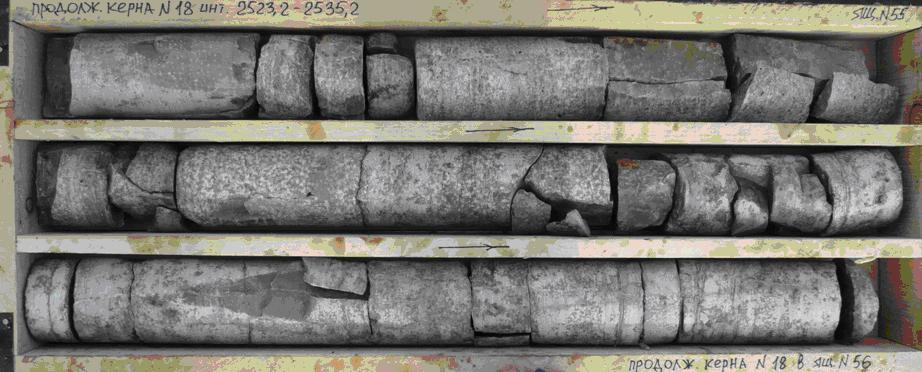
\includegraphics[scale=0.5]{images/kern.jpg}
            \caption{Пример керна}
        \end{figure}
        
        К сохранности и качеству керна предъявляются требования, обеспечивающие достоверность сведений о составе и строении вскрытых скважиной горной породы и полезных ископаемых. Сохранность керна оценивается его линейным (или объёмным) выходом — процентным отношением суммарной длины (или фактической массы) поднятого керна к длине пробуренного интервала (или расчётной массе для пробуренного интервала) скважины.
        
        В дальнейшем керн исследуется и анализируется (химический, спектральный, петрографический и другие анализы) в лаборатории с помощью различных методов и на различном оборудовании, в зависимости от того, какие данные должны быть получены.
        
        Выход керна по руде обычно колеблется от 50 до 80\%. В плотных и однородных рудах и породах он повышается до 100\%. В мягких и сильно трещиноватых рудах выход керна иногда снижается до нуля. При отсутствии или малом выходе керна в пробу поступает шлам, вследствие чего качество опробования значительно снижается. Учитывая это, следует добиваться максимального выхода бурового керна.
        
        При опробовании массивных и вкрапленных руд большой мощности применяется секционный отбор проб с длиной керна отдельной пробы 1, 2 или 3 метра, а иногда 5 метров в соответствии с методами предстоящей эксплуатации.
        
        Описание разреза начинается с общего осмотра керна (или его части) и уточнения его местоположения в разрезе скважины. Керн, поднятый и очищенный от бурового раствора, укладывают в специальные керновые ящики, изготовленные из дерева и разделенные на продольные секции. После этого проводятся исследования состава, выделение маркирующих слоёв и прочее.
        
    \subsection*{Исследование керна}
    
        Изучение нефтегазоносных скважин по керну имеет свои специфические особенности. Они заключаются в том, что по керну скважин получают в основном геологическую информацию, связанную с закономерностями вертикального строения разрезов (последовательность и характер напластования, мощность слоев, литологический состав отложений, текстурно-структурные особенности пород и т.д.).
        
        Кроме того, отбор керна в скважинах осуществляется не полностью, поэтому полученные сведения могут носить обрывочный характер и требуют глубокого анализа строения разрезов, вскрытых ранее пробуренными скважинами, и привлечения данных геофизических исследований.
        
        Осадочные толщи имеют слоистое (часто ритмичное) строение и представляют многократное и разномасштабное повторение (чередование) пород. Поэтому при осмотре и описании керновых колонок, прежде всего, выделяются слои – геологические тела, имеющие существенно однородный литологический состав (часто одинаковую окраску), обладающие ясно выраженными подошвой и кровлей и значительной толщиной (мощностью).
        
    \subsection*{Определение наличия нефти}
    
        Фотографии керна в ультрафиолетовом свете (Рис. \ref{UV}) позволяют выделить в разрезе нефтенасыщенные участки, выявить текстурные характеристики, связанные с особенностями условий осадконакопления пород. Нефтенасыщенные интервалы керна светятся в ультрафиолетовом свете в спектре от голубого до буровато-оранжевого цвета. Чем выше плотность углеводородов и насыщенность ими пород, тем больше желтых, оранжевых и коричневых цветов. \cite{paper:kern}
        
        \begin{figure}[h]
            \centering
            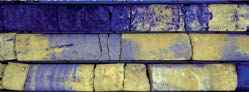
\includegraphics[scale=1]{images/UV.png}
            \caption{Фотографии керна в ультрафиолетовом свете. Неравномерное желтое свечение – неравномерно нефтенасыщенные песчаник.}
            \label{UV}
        \end{figure}        
        
        Нефтепроявления могут заключаться в выходах жидкой нефти и подъеме нефтесодержащих пород, в примазках нефти по трещинам в породах, в тонких пленках нефти на воде и т.д. Нефть может вытекать непосредственно из коренных пород, из наносов; может скапливаться в виде толстых плёнок на поверхности воды более или менее далеко от места выхода нефтеносных пород на дневную поверхность и т.д.
        
        При изучении керна иногда можно наблюдать налеты и примазки нефтяных компонентов на стенках трещин. Обычно они темноокрашенные, так как представляют собой остаточные, окисленные компоненты мигрировавших через породу нефтяных флюидов: асфальтеновых и смолисто-асфальтеновых фракций. Легкие и средние компоненты (бесцветные и светлоокрашенные) даже при интенсивном нефтяном запахе породы остаются невидимыми.
        
        Нефтесодержащие породы узнаются или сразу по цвету и запаху, если они сильно пропитаны нефтью, или после проверочных испытаний. Нефть может быть распределена в породе (например, в песчанике) равномерно или, чаще, неравномерно. В этом случае необходимо изучить характер ее распределения в зависимости от состава, структуры и текстуры.
        
        Неравномерные признаки нефтенасыщения в виде «пятнистости» по всему интервалу керна чаще всего наблюдаются в переходных зонах, ближе к водонефтяным контактам или в неоднородном пласте-коллекторе с резкой изменчивостью ёмкостно-фильтрационных свойств. В этом случае необходимо детально изучить весь интервал керна на нефтенасыщенность. \cite{paper:oil}
        
    \subsection*{Проблема}
        
        Информация о керне описывается послойно: один слой - один тип породы.
        
        В какой-то момент времени геологи поняли, что стоит детализировать описание пород: нарезали слои на фрагменты по изображениям с шагом до 1 метра и сделали для таких изображений экспертную разметку (разметка делалась несколькими экспертами, мнение которых могло не совпадать друг с другом).
        
        Недавно геологи задумались о том, что можно размечать изображения керна с большей точностью, что позволит создавать более точные модели пластов.


\section{Цели работы}

    Целью данной работы является получение описания керна на основе выборки фотографий. Описание должно включать в себя:
    
    \begin{itemize}
        \item Тип породы с точностью до 20 см. 
        \item Карбонатность с точностью до 10 см.
        \item Нефтенасыщенность с точностью до 10 см.
        \item Разрушенность с точностью до 5 см.
    \end{itemize}
    
    Также целью работы является написание удобной для пользователя обёртки над полученным решением для последующего использования.


\section{Постановка задачи}

    Для достижения приведённых целей были поставлены следующие задачи:
    
    \begin{itemize}
        \item Произвести разведочный анализ предоставленных данных
        \item Ознакомиться с возможными решениями
        \item Реализовать решения и найти лучшие
        \item Сравнить результаты с уже имеющимися у заказчика
        \item Создать оболочку для удобного использования решения
    \end{itemize}    
    

\section{Исходные данные}

    В качестве исходных данных были предоставленны фотографии керна и те же самые фотографии керна, но в ультрафиолетовом освещении (Рис. \ref{sample}).
    
    \begin{figure}[h]
        \centering
        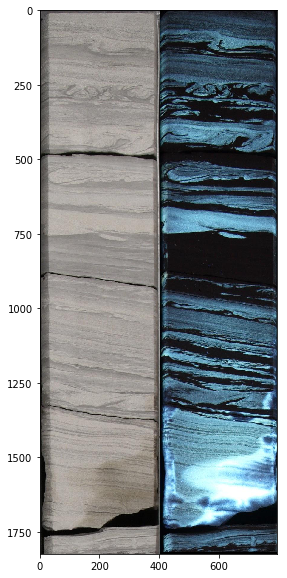
\includegraphics[scale=0.4]{images/sample.png}
        \caption{Пример из исходных данных. Слева — фото керна, справа — фото того же керна, но в УФ.}
        \label{sample}
    \end{figure}       
    
    К фотографиям была предоставлена таблица (Таблица \ref{sample_table}) с описанием каждой фотографии. Нам необходимо предсказывать последние 4 параметра — \textbf{Rock} (тип породы), \textbf{Carbonate} (карбонатность), \textbf{Ruin} (разрушенность), \textbf{Saturation} (нефтенасыщенность). 
        
    Как было сообщено заказчиком, тестовая выборка будет состоять из фотографий и таблицы с двумя полями: \textbf{PhotoTop}, \textbf{PhotoDown}. Таким образом, избавимся от ненужных записей и получим таблицу (Таблица \ref{sample_table_cleaned}).
    
    \begin{table}[h!]
        \centering
        \begin{tabular}{|l|l|l|}
            \hline
            {} &                0 &                1 \\
            \hline
            Folder         &          Unload1 &          Unload1 \\
            Id             &          1000000 &          1000001 \\
            Field          &           Field6 &           Field6 \\
            Well           &           Well11 &           Well11 \\
            CoringTop      &           1957.1 &           1957.1 \\
            CoringDown     &           1963.1 &           1963.1 \\
            CoringTopBind  &           1958.3 &           1958.3 \\
            CoringDownBind &           1964.3 &           1964.3 \\
            CoreRecovery   &             5.93 &             5.93 \\
            PhotoTop       &                0 &                0 \\
            PhotoDown      &                1 &                1 \\
            PhotoType      &               ДС &               УФ \\
            LayerTop       &                0 &                0 \\
            LayerDown      &             1.45 &             1.45 \\
            Rock           &         песчаник &         песчаник \\
            Carbonate      &   не карбонатный &   не карбонатный \\
            Ruin           &      не разрушен &      не разрушен \\
            Saturation     &  нефтенасыщенные &  нефтенасыщенные \\
            \hline
        \end{tabular}
        \caption{Пример из таблицы исходных данных. Предоставлена информация о первых двух записях — один и тот же керн, обычная фотография и фотография в УФ.}
        \label{sample_table}  
        \vspace*{2 cm}
    \end{table}

    \begin{table}[h!]
        \centering
        \begin{tabular}{|l|l|l|}
            \hline
            {} &                0 &                1 \\
            \hline
            Id             &          1000000 &          1000001 \\
            PhotoTop       &                0 &                0 \\
            PhotoDown      &                1 &                1 \\
            Rock           &         песчаник &         песчаник \\
            Carbonate      &   не карбонатный &   не карбонатный \\
            Ruin           &      не разрушен &      не разрушен \\
            Saturation     &  нефтенасыщенные &  нефтенасыщенные \\
            \hline
        \end{tabular}
        \caption{После удаления ненужных столбцов.}
        \label{sample_table_cleaned}  
        \vspace*{2 cm}
    \end{table}   
    
    \FloatBarrier
    
    \subsection{Анализ данных}
        
        Поля \textbf{PhotoUp} и \textbf{PhotoDown} означают начало и конец данной фотографии в данном образце керна. В нашем примере \textbf{PhotoUp}=0 и \textbf{PhotoDown}=1. Это значит, что длина керна на фотографии — 1 метр.
        
        \subsubsection*{Распределение данных}
        
        
        В категории \textbf{Rock} очень много значений, которые имеют малое количество экземпляров в сравнении с другими категориями, поэтому выбросим их. Итоговое распределение фотографий для категории \textbf{Rock}:
        
        \begin{table}[h!]
            \centering
            \begin{tabular}{|l|c|}
                \hline
                \textbf{тип породы} & \textbf{количество экземпляров} \\
                \hline
                песчаник            & 2482                            \\
                \hline
                аргиллит            & 1220                            \\
                \hline
                алевролит           & 1138                            \\
                \hline
                переслой            & 686                            \\
                \hline
            \end{tabular}
            \caption{Распределение категории "тип породы".}
            \label{table_rock}  
        \end{table}  
        
        В категории \textbf{Carbonate} всё оставим, как есть:
        
        \begin{table}[h!]
            \centering
            \begin{tabular}{|l|c|}
                \hline
                \textbf{карбонатность}            & \textbf{количество экземпляров} \\
                \hline
                не карбонатный                    &       4056 \\
                \hline
                с карб. обломками или конкрециями &       1292 \\
                \hline
                слабокарбонатный                  &        298 \\
                \hline
                сильнокарбонатный                 &        246 \\
                \hline
                пятнисто карбонатный              &        226 \\
                \hline
                среднекарбонатный                 &        196 \\
                \hline
                с примесью                        &        100 \\
                \hline
            \end{tabular}    
            \caption{Распределение категории "карбонатность".}
            \label{table_carbonate}  
        \end{table}      
        
        Категория \textbf{Ruin}:
        
        \begin{table}[h!]
            \centering
            \begin{tabular}{|l|c|}
                \hline
                \textbf{разрушенность}            & \textbf{количество экземпляров} \\
                \hline
                частично разрушен &  3132 \\
                \hline
                не разрушен       &  2944 \\
                \hline
                разрушен          &   338 \\
                \hline
            \end{tabular}    
            \caption{Распределение категории "разрушенность".}
            \label{table_ruin}
        \end{table}
        
        \vskip 0.2in
        
        Категория \textbf{Saturation}:
        
        \begin{table}[h!]
            \centering
            \begin{tabular}{|l|c|}
                \hline
                \textbf{насыщенность}            & \textbf{количество экземпляров} \\
                \hline
                не опред.                &        4596 \\
                \hline
                нефтенасыщенные          &         668 \\
                \hline
                пятнисто нефтенасыщенные &         358 \\
                \hline
                битуминозный             &         350 \\
                \hline
                продукт                  &         326 \\
                \hline
                слабо нефтенасыщенные    &         116 \\
                \hline
            \end{tabular}    
            \caption{Распределение категории "насыщенность".}
            \label{table_saturation}  
        \end{table} 
    
    
 




\section{Решение}
    
    Данную задачу можно решать двумя принципиально разными способами: сегментацией и классификацией.

    \subsection{Сегментация изображения}
    
        При сегментации изображения мы получаем на выходе картинку, на которой каждый слой отмечен своим цветом (Рис. \ref{segmentation}). 
        
        \begin{figure}[h]
            \centering
            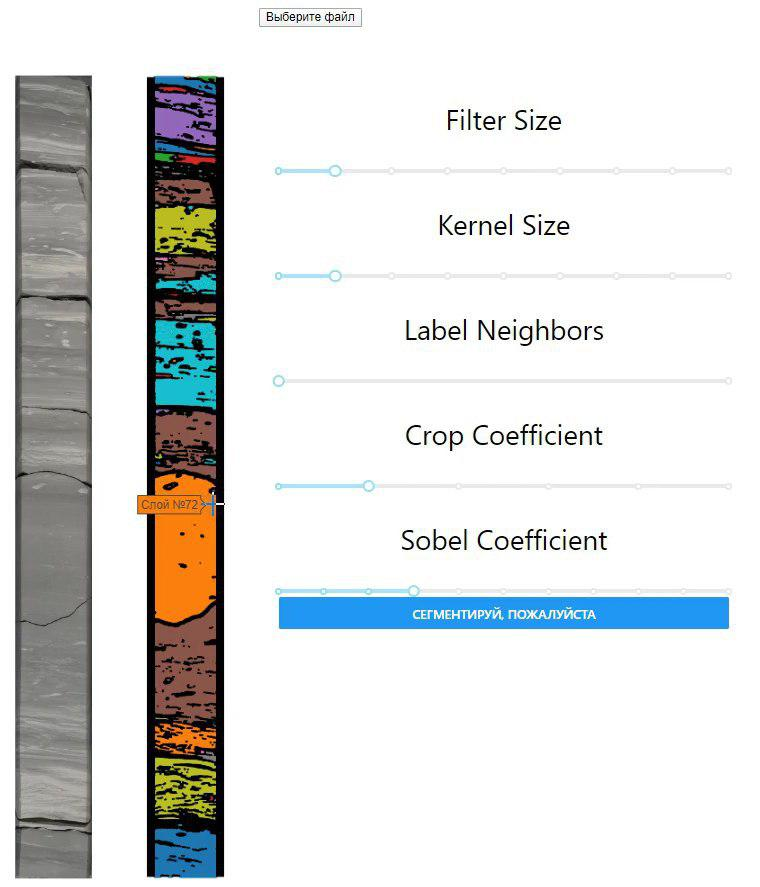
\includegraphics[scale=0.35]{images/segmentation.jpg}
            \caption{Пример работы сегментационного алгоритма.}
            \label{segmentation}
        \end{figure}
        
        Большим плюсом такого подхода является точность, ведь мы классифицируем каждый пиксель входного изображения. Изучив статью \cite{paper:segmentation}, посвящённую задачи сегментации, понял, что для обучения потребуются данные, в которых каждый пиксель размечен под определённую категорию. Так как этот процесс ресурсозатратный, было принято решение перейти к рассмотрению следующих подходов и вернуться к сегментации в дальнейшем.
    
    \subsection{Классификация изображения}
    
        При решении задачи классификации мы заранее обучаем модель на размеченных данных. Размеченные данные у нас имеются, осталось решить вопрос с точностью предсказания. Напомню, что для разных категорий мы должны предсказывать значение с разной точностью. Таким образом, мы приходим к тому, чтобы фотографию керна разбивать на более мелкие. Попробуем загрузить предобученную модель для выделения признаков VGG16, разморозить последние слои, переобучить модель и посмотреть на результаты:
    
        \begin{figure}[h]
            \centering
            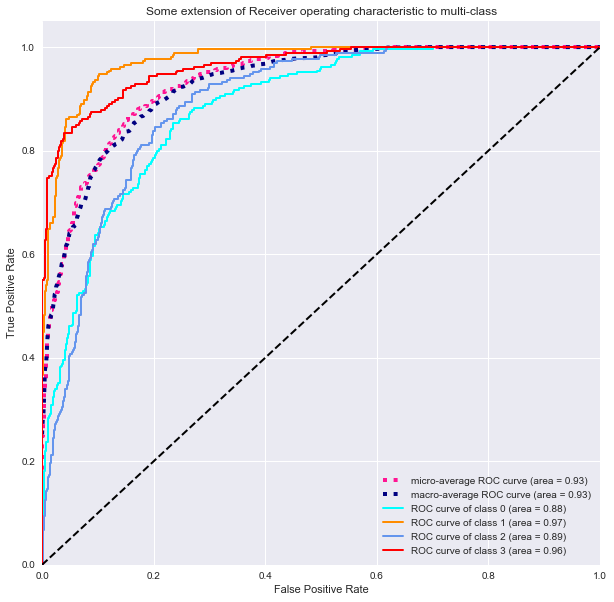
\includegraphics[scale=0.6]{images/auc.png}
            \caption{VGG16 ROC AUC.}
            \label{auc}
        \end{figure}    
        
        Top-1 accuracy вышла 0.75, что очень даже неплохо, учитывая, что мы используем только половину информации (модель обучена и проверена на не ультрафиолетовых фотографиях). В теории, данный подход может дать ещё большую точность, если эту модель совместить с моделью для классификации по УФ фотографиям.
    
    \subsection{Метрическая классификация изображения}
        
        Был разобран другой подход к классификации изображений — на основе расстояния \cite{paper:oneshot}. Планирую протестировать его и сравнить результаты.

\section*{Заключение}

    Что было сделано в рамках данной работы:
    
    \begin{itemize}
        \item Изучена предметная область
        \item Провёдены изучение и подготовка данных
        \item Провёден разбор возможных решений
        \item Реализовано одно решение 
    \end{itemize}      
        
    Что планируется сделать:
    
    \begin{itemize}
        \item Улучшить реализованное решение
        \item Реализовать метрическую классификацию
        \item Реализовать сегментацию
        \item Сравнить результаты между собой
        \item Обернуть решение в удобный интерфейс
    \end{itemize}      


\setmonofont[Mapping=tex-text]{CMU Typewriter Text}
\bibliographystyle{ugost2008ls}
\bibliography{diploma.bib}
\end{document}